\documentclass{article}

\usepackage[T2A]{fontenc}
\usepackage[utf8]{inputenc}
\usepackage[russian]{babel}
\usepackage{commath}
\usepackage{amsmath}
\usepackage{amsfonts} 
\usepackage{parskip}
\usepackage{color}
\usepackage{hyperref}
\usepackage{titling}
\usepackage{graphicx}
\usepackage[a4paper, left=2.5cm, right=1.5cm, top=2.5cm, bottom=2.5cm]{geometry}

\graphicspath{ {./images/} }
\setlength{\droptitle}{-3cm}
\hypersetup{
    colorlinks=true, %set true if you want colored links
    linktoc=all,     %set to all if you want both sections and subsections linked
    linkcolor=blue,  %choose some color if you want links to stand out
}

\pagenumbering{arabic}

\begin{document}
\title{Числовые последовательности и их пределы}
\author{Ученик 10-4 класса Паньков М.А. по лекции к.ф.-м.н. Протопоповой Т.В.}
\date{от 16 марта 2021 г.}
\maketitle

\addtocontents{toc}{\protect\contentsline{section}{\protect\numberline{}Числовые последовательности и их пределы}{}{}}
\section{Лекция №21}

\textbf{Определение.} Будем говорить, что \( x_n \) сходится к \( a(\lim_{n \to \infty} x_n = a) \), если \( \forall \varepsilon > 0 \ \exists \  N = N(\varepsilon): \forall n > N,\ \abs{x_n - a} < \varepsilon \)

\textbf{Геометрический смысл:}\\
a --- предел \( x_n \), \(a - \varepsilon < x_n < a + \varepsilon\)\\
\(O_a = (a - \varepsilon,\ a + \varepsilon)\) --- \(\varepsilon\)-окрестность т. a


\includegraphics[scale=0.5]{21_0}\\
\textbf{Примеры:}
\begin{enumerate}
    \item Док-ть \(\lim_{n \to \infty} \frac{1}{n} = 0\)
    
    \( \forall \varepsilon > 0 \ \exists \  N = N(\varepsilon): \forall n > N,\ \textrm{док-ть: }\abs{\frac{1}{n} - 0} < \varepsilon \)
    \\\(\abs{\frac{1}{n} - 0} = \abs{\frac{1}{n}} = \frac{1}{n} < \varepsilon, \ n > \frac{1}{\varepsilon} \Rightarrow N = \frac{1}{\varepsilon}\)
    \\\(N = [\frac{1}{\varepsilon}] + 1 \in \mathbb{N}\)([x] --- выделение целой части)
    
    \([x] \leq x < [x] + 1\)
    \\\(\frac{1}{[x]+1} < \frac{1}{x}\)

    действительно:
    \\\(\frac{1}{n} < \frac{1}{N} = \frac{1}{[\frac{1}{\varepsilon}]+1} < \frac{1}{\frac{1}{\varepsilon}} = \varepsilon\), ч.т.д.
    \item Док-ть \(\lim_{n \to \infty} \frac{n}{n+1} = 1\)
    \\\( \forall \varepsilon > 0 \ \exists \  N = N(\varepsilon): \forall n > N,\ \textrm{док-ть: }\abs{\frac{n}{n+1} - 1} < \varepsilon \)
    \\\(\abs{\frac{n}{n+1} - 1} = \abs{\frac{n-n-1}{n+1}} = \frac{1}{n+1} < \frac{1}{n} < \varepsilon\), ч.т.д. (\(N = [\frac{1}{\varepsilon} - 1] + 1\))

    %\(x_n = \frac{1}{n} \longrightarrow_{n \to \infty} 0\)
    \item \(\alpha\) --- б.д.д.
    \\\(\alpha_n\) --- приближение б.д.д. по недостатку с точностью до \(\frac{1}{10^n}\)
    \\Покажем, что \(\alpha_n \longrightarrow_{n \to \infty} \alpha\)
    \\\(\forall \varepsilon > 0 \ \exists \ N : \forall n > N, \ \abs{\alpha_n-\alpha} < \varepsilon\)
    \\\(\abs{\alpha_n - \alpha} = \abs{a, \ a_1, \ a_2, ..., \ a_n - a, \ a_1, \ a_2, ..., \ a_n, \ a_{n+1}, \ a_{n+2}....} = 0, \underbrace{0\  .... \ 0}_n, \ a_{n+1}, \ a_{n+2}.... < \frac{1}{10^n} < \frac{1}{9n} < \ <\varepsilon\)
    \\\(10^n = (1+9)^n > 9n\) \qquad \(n > \frac{1}{9\varepsilon}\)
    \\\(N = [\frac{1}{9\varepsilon}] + 1\)

    Сходимость может быть разной

    \(x_n = \frac{1}{n}\)
    \qquad 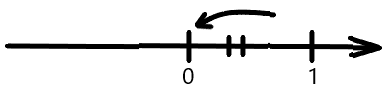
\includegraphics[scale=0.3]{22_0}

    \(x_n = -\frac{1}{n}\)
    \qquad 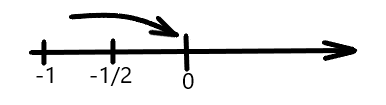
\includegraphics[scale=0.3]{22_1}

    \(x_n = \frac{(-1)^n}{n}\)
    
\end{enumerate}
\end{document}